\subsection[Declarative vs Imperative]{Declarative vs Imperative Programming}

\frame{\tableofcontents[currentsection, currentsubsection]}

\begin{frame}{Declarative vs imperative programming}
	\hhl{Declarative programming}:
	\begin{itemize}
		\item Program describes \hl{logic} rather than \hl{control flow}
		\item Program describes \hl{\enquote{what}} rather than \hl{\enquote{how}}
		%\item Focus on \hl{description} rather than \hl{implementation}
		\item Aims for correspondence with mathematical logic
		\item \hl{FP} is usually considered a subcategory
	\end{itemize}
	
	\medskip
	Opposite: \hhl{imperative programming}:
	\begin{itemize}
		\item Algorithms as a sequence of steps
		\item Often used synonymously: \hhl{procedural programming} \srem{(emphasizing the concept of using procedure calls (functions) to structure the program in a modular fashion)}
		\item \hl{OOP} is usually considered a subcategory
	\end{itemize}
\end{frame}

\begin{frame}{Examples}
	Picture book examples:
	\begin{itemize}
		\item \proglang{SQL} \srem{(Structured Query Language -- language to interact with databases $\lra$ \mauthor{Emil Kleszcz})}:
		%
		\begin{center}
			\mintinline{SQL}{SELECT * FROM Customers WHERE Country='Mexico';}
		\end{center}
		\item \hhl{Markup languages}, like \proglang{HTML}, \proglang{CSS} \srem{(Cascading Style Sheets -- language to describe styling of e.g. HTML pages)}, \dots
		%
		\begin{center}
			\mintinline{HTML}{<h1 style="color:blue;">This is a Blue Heading</h1>
			}
		\end{center}
		\item Functional programming languages like \proglang{Haskell} \srem{(even though they allow some \enquote{encapsulated} imperative parts)}
		\item \dots
\end{itemize}
\end{frame}
%
\begin{frame}{Powerful backends I}
	Idea:
	\begin{itemize}
		\item Split up your code into \hhl{application/analysis specific code} \srem{(describing the problem)} and a \hhl{backend/library} \srem{(implementing solution strategies)}
		\item The application specific code starts to \emph{feel} very \hhl{declarative}
		\item The backend can use different strategies depending on the nature/scale of the problem
	\end{itemize}

	\medskip
	Example:
	\inputminted{python}{code/paradigms/dp/py_pandas.py}
\end{frame}
%
%
\begin{frame}{Powerful backends II}
	\begin{itemize}
		\item However, we want more of our backend, e.g. delayed or distributed execution
		\item \texttt{pandas} can also be viewed as a \enquote{declarative language} describing the problem $\lra$ have a more sophisticated backend handle all operations $\lra$ \texttt{modin pandas}
		
		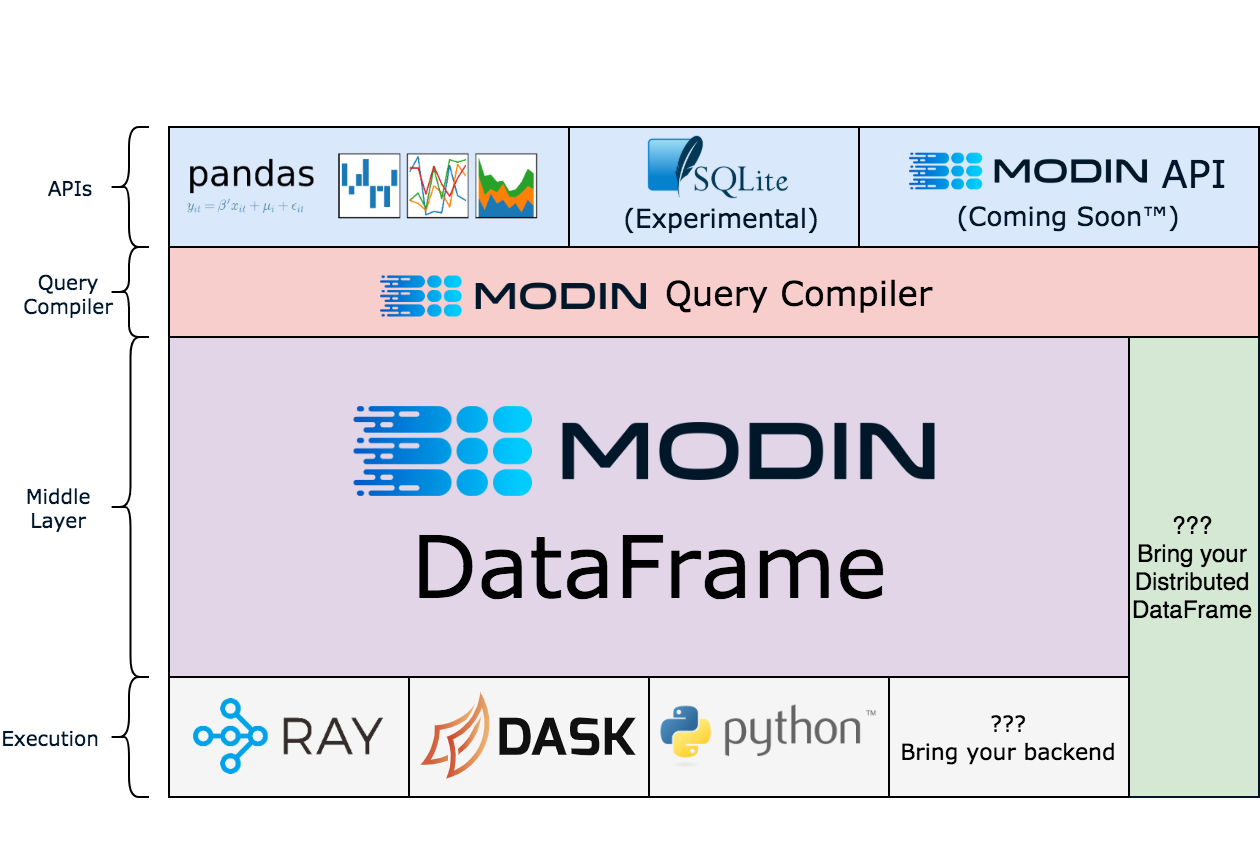
\includegraphics[width=8cm, trim=0cm 2.5cm 0cm 2.5cm, clip]{figures/paradigms/dp/modin_architecture.png}
		%
%		\item \proglang{ROOT} can also do dataframes: \texttt{RDataFrame}
	\end{itemize}
\end{frame}
%
\begin{frame}{Powerful backends III}
	Belle II steering file:
	\inputminted{python}{code/paradigms/dp/belle2_steering_file.py}
	%Many new things coming specifically for HEP, e.g. LINQToROOT
\end{frame}
%
\begin{frame}{Powerful backends IV}
	Many more powerful tools coming, e.g.
	\smallskip 
	\begin{itemize}
		\item LINQtoROOT: Uses \proglang{C\#} with \proglang{LINQ} queries to describe problem
		\inputminted[fontsize=\small]{csharp}{code/paradigms/dp/linqtoroot.cs}
		\item The FAST HEP toolkit: Uses yaml config files to describe problem; using pandas, numpy, etc. in the backend
		\inputminted[fontsize=\small]{yaml}{code/paradigms/dp/fast.yaml}
		\item Many more\dots
	\end{itemize}
\end{frame}